\begin{figure}[ht]
	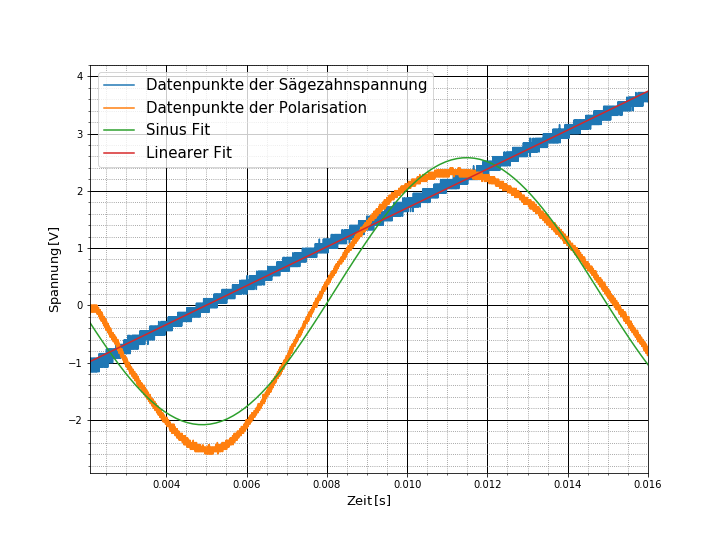
\includegraphics[scale=0.5]{Bild/SinusProblem}
	\centering
	\caption[Sinus Fit an die Messpunkte Versuchsteil 1]{Sinus Fit für Versuchsteil 1. Es ist klar erkennbar, dass die Maxima, an denen man interessiert ist, nicht in der nähe der Messpunkte liegen.}
	\label{ProbelmSinus}
\end{figure}
\begin{figure}[ht]
	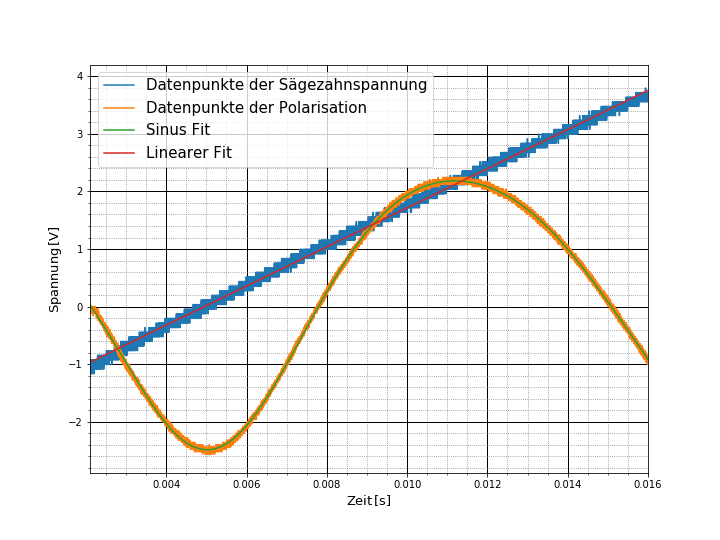
\includegraphics[scale=0.5]{Bild/V1_2}
	\centering
	\caption[Plot zu Versuchsteil 1 Nr.2]{Datenpunkte der ersten Messmethode mit Hilfe der Sägezahnspannung. Grüner Fit mit Hilfe eines Polynoms neunter Ordnung.}
\end{figure}
\begin{figure}[ht]
	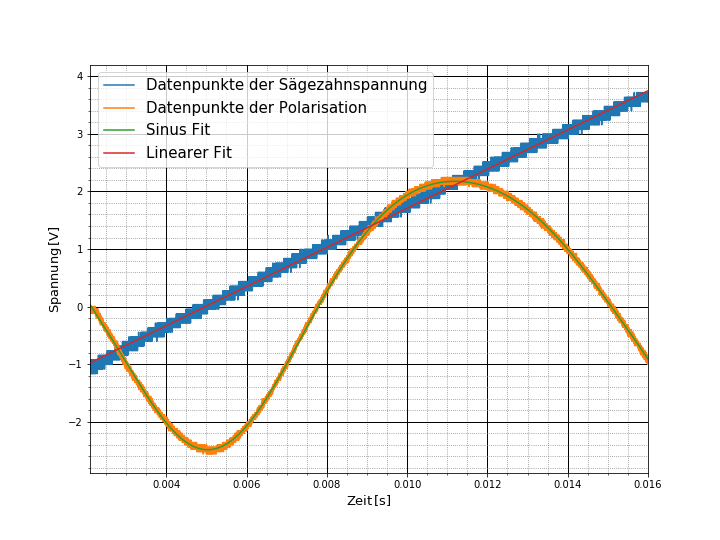
\includegraphics[scale=0.5]{Bild/V1_3}
	\centering
	\caption[Plot zu Versuchsteil 1 Nr.3]{Datenpunkte der ersten Messmethode mit Hilfe der Sägezahnspannung. Grüner Fit mit Hilfe eines Polynoms neunter Ordnung.}
\end{figure}
\begin{figure}[ht]
	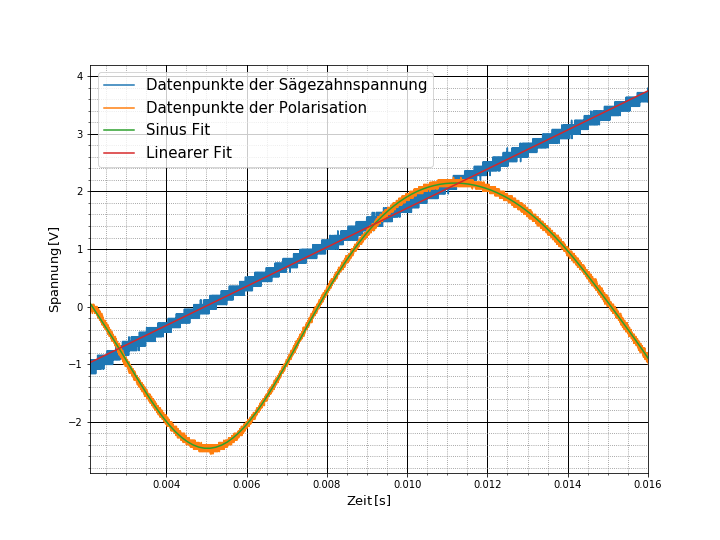
\includegraphics[scale=0.5]{Bild/V1_4}
	\centering
	\caption[Plot zu Versuchsteil 1 Nr.4]{Datenpunkte der ersten Messmethode mit Hilfe der Sägezahnspannung. Grüner Fit mit Hilfe eines Polynoms neunter Ordnung.}
\end{figure}
\begin{figure}[ht]
	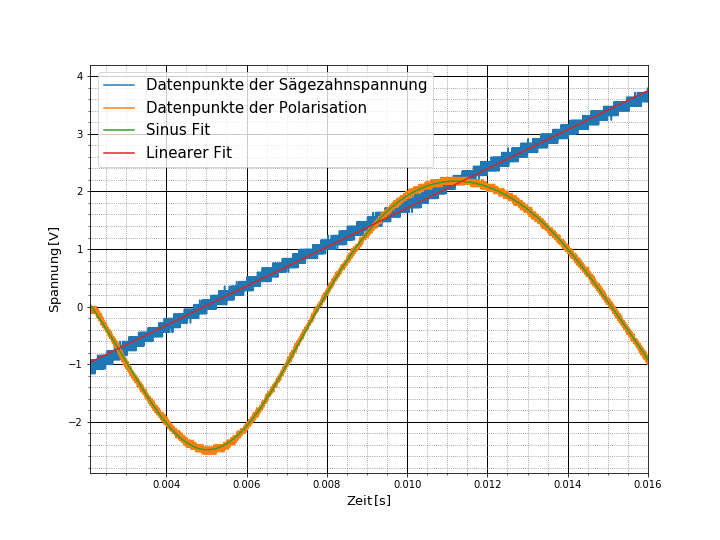
\includegraphics[scale=0.5]{Bild/V1_5}
	\centering
	\caption[Plot zu Versuchsteil 1 Nr.5]{Datenpunkte der ersten Messmethode mit Hilfe der Sägezahnspannung. Grüner Fit mit Hilfe eines Polynoms neunter Ordnung.}
\end{figure}
\begin{figure}[ht]
	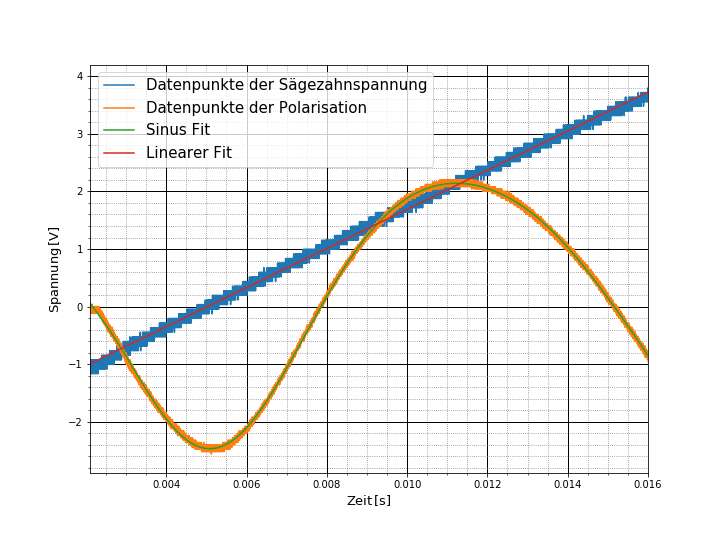
\includegraphics[scale=0.5]{Bild/V1_6}
	\centering
	\caption[Plot zu Versuchsteil 1 Nr.6]{Datenpunkte der ersten Messmethode mit Hilfe der Sägezahnspannung. Grüner Fit mit Hilfe eines Polynoms neunter Ordnung.}
\end{figure}
\begin{figure}[ht]
	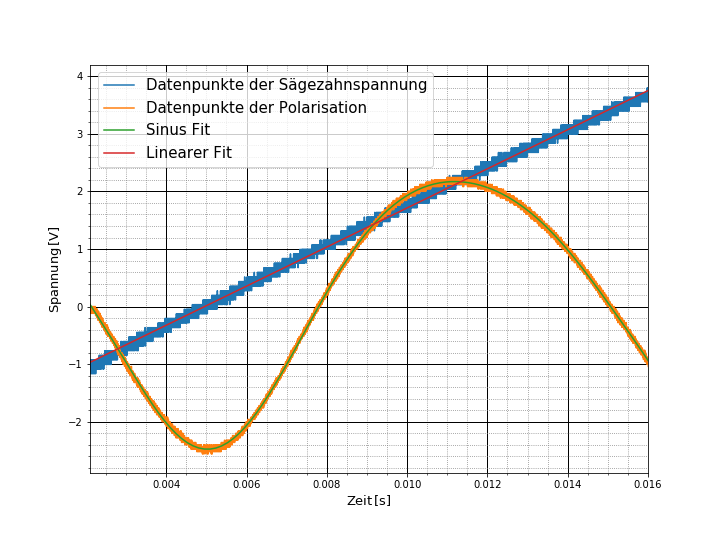
\includegraphics[scale=0.5]{Bild/V1_7}
	\centering
	\caption[Plot zu Versuchsteil 1 Nr.7]{Datenpunkte der ersten Messmethode mit Hilfe der Sägezahnspannung. Grüner Fit mit Hilfe eines Polynoms neunter Ordnung.}
\end{figure}
\begin{figure}[ht]
	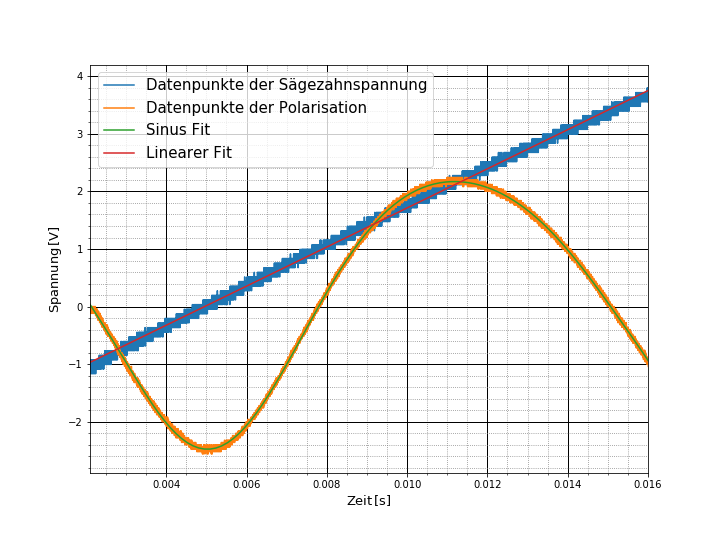
\includegraphics[scale=0.5]{Bild/V1_8}
	\centering
	\caption[Plot zu Versuchsteil 1 Nr.8]{Datenpunkte der ersten Messmethode mit Hilfe der Sägezahnspannung. Grüner Fit mit Hilfe eines Polynoms neunter Ordnung.}
\end{figure}
\begin{figure}[ht]
	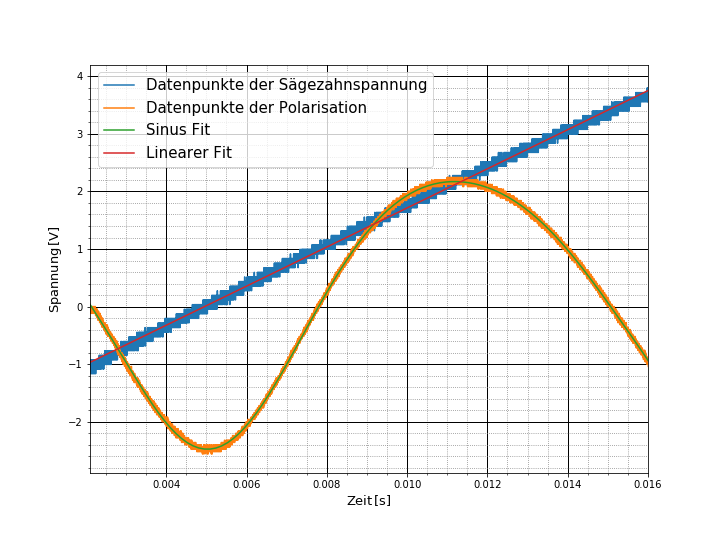
\includegraphics[scale=0.5]{Bild/V1_9}
	\centering
	\caption[Plot zu Versuchsteil 1 Nr.9]{Datenpunkte der ersten Messmethode mit Hilfe der Sägezahnspannung. Grüner Fit mit Hilfe eines Polynoms neunter Ordnung.}
\end{figure}
\begin{figure}[ht]
	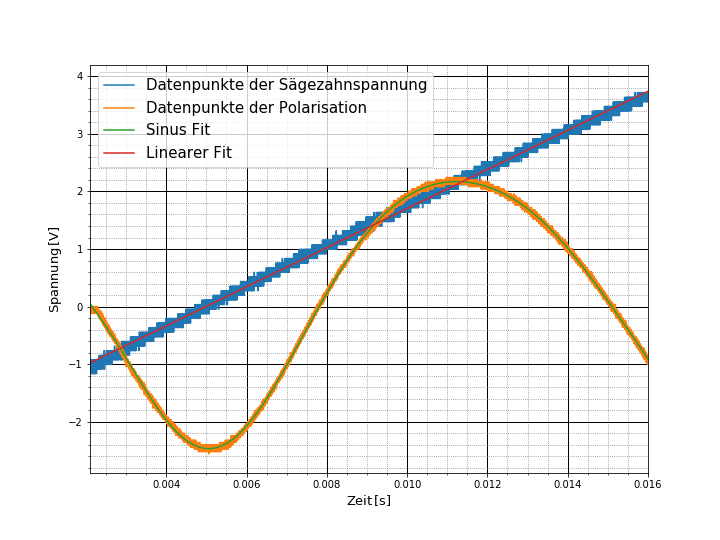
\includegraphics[scale=0.5]{Bild/V1_10}
	\centering
	\caption[Plot zu Versuchsteil 1 Nr.10]{Datenpunkte der ersten Messmethode mit Hilfe der Sägezahnspannung. Grüner Fit mit Hilfe eines Polynoms neunter Ordnung.}
\end{figure}
\begin{figure}[ht]
	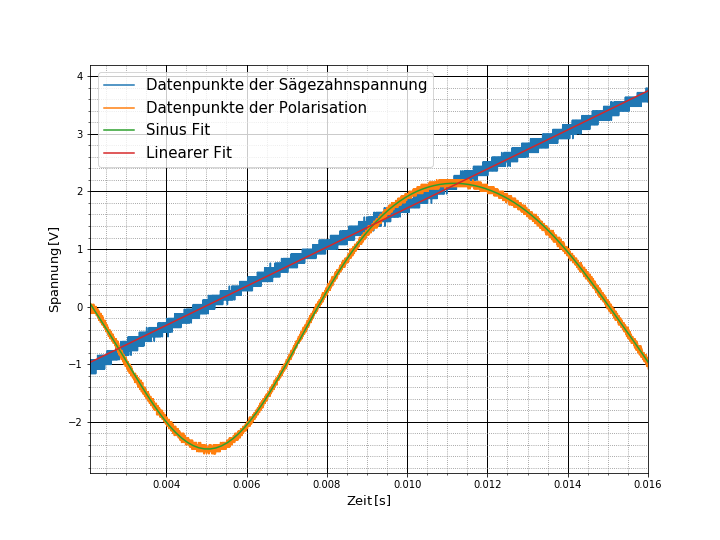
\includegraphics[scale=0.5]{Bild/V1_11}
	\centering
	\caption[Plot zu Versuchsteil 1 Nr.11]{Datenpunkte der ersten Messmethode mit Hilfe der Sägezahnspannung. Grüner Fit mit Hilfe eines Polynoms neunter Ordnung.}
\end{figure}
\begin{figure}[ht]
	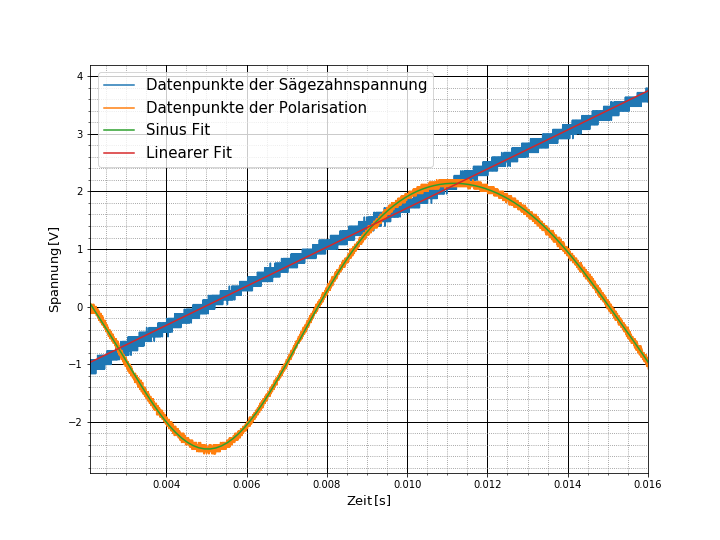
\includegraphics[scale=0.5]{Bild/V1_12}
	\centering
	\caption[Plot zu Versuchsteil 1 Nr.12]{Datenpunkte der ersten Messmethode mit Hilfe der Sägezahnspannung. Grüner Fit mit Hilfe eines Polynoms neunter Ordnung.}
\end{figure}
\begin{figure}[ht]
	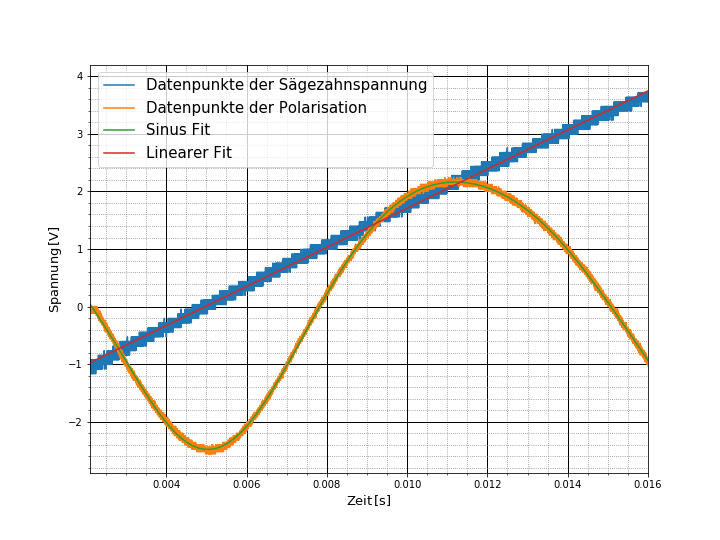
\includegraphics[scale=0.5]{Bild/V1_13}
	\centering
	\caption[Plot zu Versuchsteil 1 Nr.13]{Datenpunkte der ersten Messmethode mit Hilfe der Sägezahnspannung. Grüner Fit mit Hilfe eines Polynoms neunter Ordnung.}
\end{figure}
\begin{figure}[ht]
	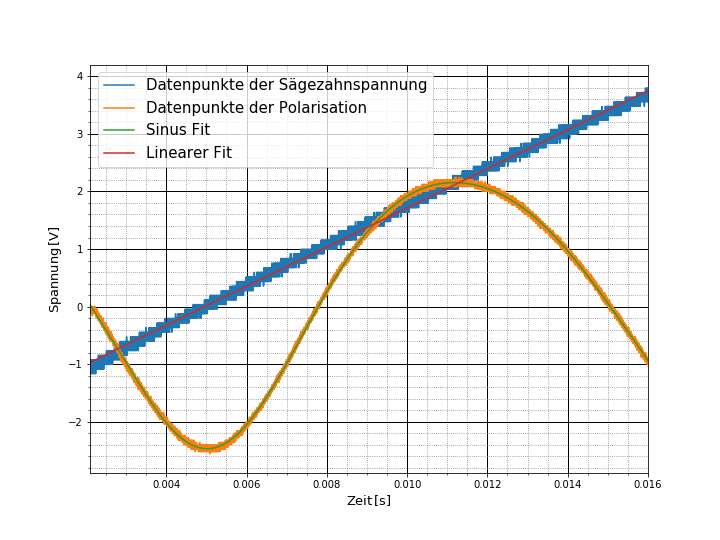
\includegraphics[scale=0.5]{Bild/V1_14}
	\centering
	\caption[Plot zu Versuchsteil 1 Nr.14]{Datenpunkte der ersten Messmethode mit Hilfe der Sägezahnspannung. Grüner Fit mit Hilfe eines Polynoms neunter Ordnung.}
\end{figure}
\begin{figure}[ht]
	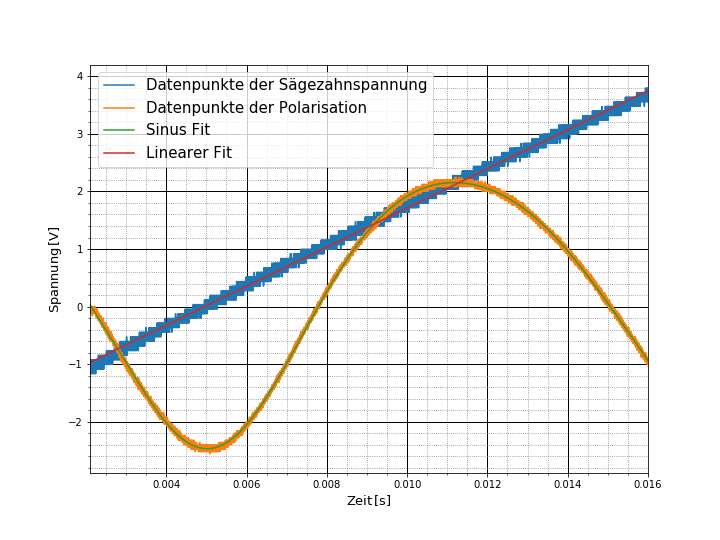
\includegraphics[scale=0.5]{Bild/V1_15}
	\centering
	\caption[Plot zu Versuchsteil 1 Nr.15]{Datenpunkte der ersten Messmethode mit Hilfe der Sägezahnspannung. Grüner Fit mit Hilfe eines Polynoms neunter Ordnung.}
\end{figure}
\FloatBarrier
\subsection{Versuchsprotokoll}
\FloatBarrier
\begin{figure}[ht]
	\centering
	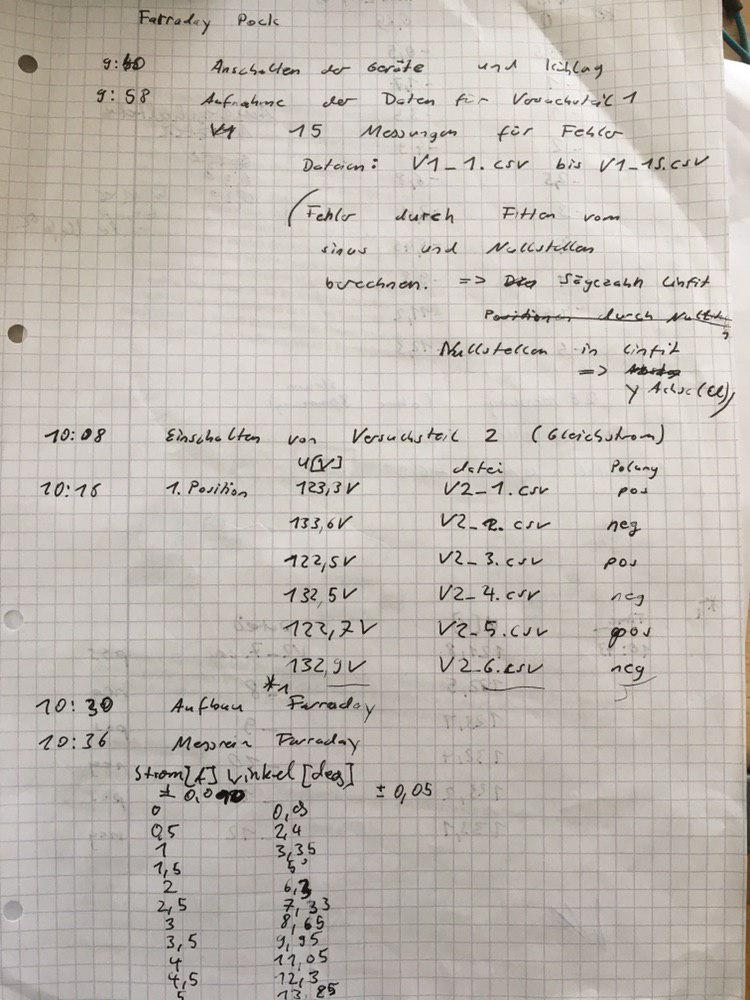
\includegraphics[scale=0.5]{Bilder/protokoll_1}
\end{figure}
\begin{figure}[ht]
	\centering
	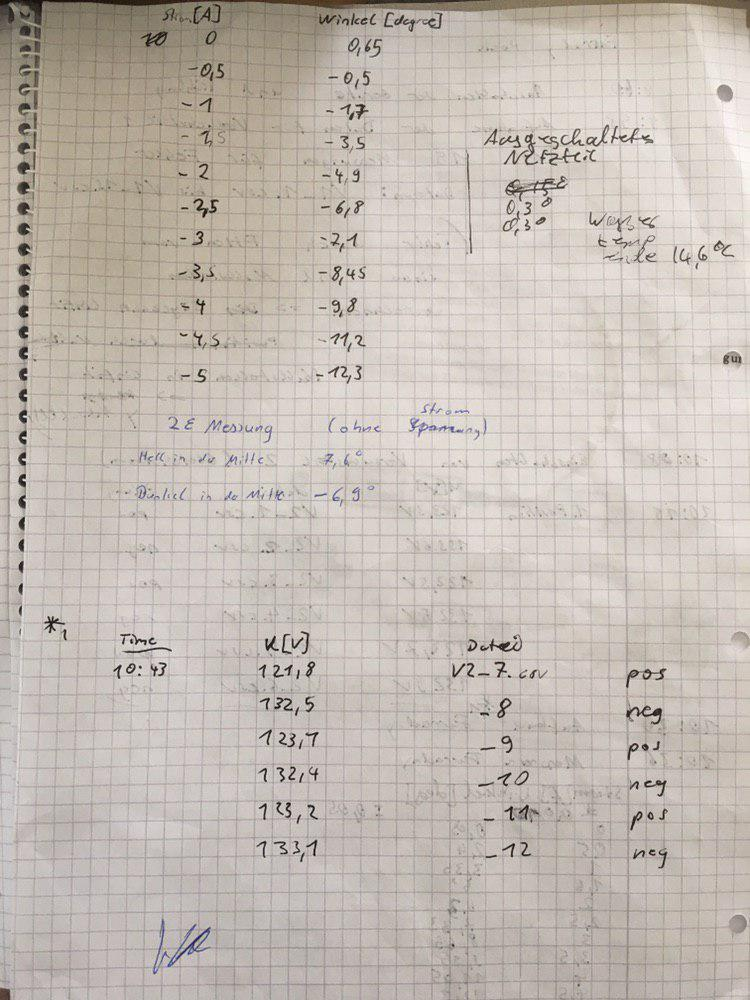
\includegraphics[scale=0.5]{Bilder/protokoll_2}
\end{figure}